\documentclass[11pt]{article}
\usepackage{amsmath,amsbsy,amssymb,verbatim,fullpage,ifthen,graphicx,bm,amsfonts,amsthm,url}
\usepackage{graphicx}
\usepackage{xcolor}
%\usepackage[dvipsnames]{xcolor}
\usepackage{algpseudocode}
\newcommand{\mfile}[1]  {{\small \verbatiminput{./#1}}} % Jeff Fessler, input matlab file
\newcommand{\tmop}[1]{\ensuremath{\operatorname{#1}}}
\newcommand{\R}{\mathbb{R}}
\newcommand{\C}{\mathbb{C}}
\newcommand{\Z}{\mathbb{Z}}
\newcommand{\A}{\mathcal{A}}
\newcommand{\minimize}{\operatorname*{minimize\ }}
\newcommand{\maximize}{\operatorname*{maximize}}
\newcommand{\opdet}[1]{\operatorname{\textbf{det}}\left(#1\right)}
\newcommand{\optr}[1]{\operatorname{\textbf{tr}}\left(#1\right)}
\newcommand{\answer}[2][blue]{\ifdefined\AnswerDefine{\color{#1}\it#2}\fi}
\newcommand{\mtx}[1]{\mathbf{#1}}
\newcommand{\vct}[1]{\mathbf{#1}}
\def \lg       {\langle}
\def \rg       {\rangle}
\def \mA {\mtx{A}}
\def \mB {\mtx{B}}
\def \mI {\mtx{I}}
\def \mJ {\mtx{J}}
\def \mU {\mtx{U}}
\def \mS {\mtx{S}}
\def \mV {\mtx{V}}
\def \mW {\mtx{W}}
\def \mLambda {\mtx{\Lambda}}
\def \mSigma {\mtx{\Sigma}}
\def \mX {\mtx{X}}
\def \mY {\mtx{Y}}
\def \mZ {\mtx{Z}}
\def \zero     {\mathbf{0}}
\def \vzero    {\vct{0}}
\def \vone    {\vct{1}}
\def \vu {\vct{u}}
\def \vv {\vct{v}}
\def \vx {\vct{x}}
\def \vy {\vct{y}}
\def \vz {\vct{z}}
\def \vphi {\vct{\phi}}
\def \vmu {\vct{\mu}}
\def \R {\mathbb{R}}


\usepackage{xspace}
\makeatletter
\DeclareRobustCommand\onedot{\futurelet\@let@token\@onedot}
\def\@onedot{\ifx\@let@token.\else.\null\fi\xspace}

\def\eg{\emph{e.g}\onedot} \def\Eg{\emph{E.g}\onedot}
\def\ie{\emph{i.e}\onedot} \def\Ie{\emph{I.e}\onedot}
\def\cf{\emph{c.f}\onedot} \def\Cf{\emph{C.f}\onedot}
\def\etc{\emph{etc}\onedot} \def\vs{\emph{vs}\onedot}
\def\wrt{w.r.t\onedot} \def\dof{d.o.f\onedot}
\def\etal{\emph{et al}\onedot} \def\st{\emph{s.t}\onedot}
\pagestyle{plain}

\title{{\bf Homework Set 3, CPSC 8420, Fall 2024}} % Change to the appropriate homework number
\author{\Large\underline{Your Name}}
\date{\textbf{\Large\textcolor{red}{Due 11/11/2024, 11:59PM EST}}} % put your name in the LastName, FirstName format
%\date{\today}

\begin{document}
	\maketitle
	

	%\section*{Problem 1}
\section*{Problem 1}
Please download the image from \url{https://en.wikipedia.org/wiki/Lenna#/media/File:Lenna_(test_image).png} with dimension $512\times512\times3$. Assume for each RGB channel data $X$, we have $[U,\Sigma,V]=svd(X)$. Please show each compression ratio and reconstruction image if we choose first $2, 5, 20, 50,80,100$ components respectively. Also please determine the best component number to obtain a good trade-off between data compression ratio and reconstruction image quality. (Open question, that is your solution will be accepted as long as it's reasonable.)


\textbf{Answer:}

In this problem, I created a Python program that used Principal Component Analysis (PCA) on the Lenna image to explore the trade-off between data compression and image quality. 
The image was loaded and preprocessed by normalizing the pixel values to a range of [0, 1] and centering the data by subtracting the mean for each RGB channel. 
PCA was then applied independently to each of the three color channels (Red, Green, and Blue). Singular Value Decomposition (SVD) was then performed on each channel, decomposing it into matrices \( U \), \( \Sigma \), and \( V \), 
where \( \Sigma \) contains the singular values in decreasing order. 
For each channel, I reconstructed the image using a varying number of principal components (2, 5, 20, 50, 80, and 100). 
This reconstruction process involved keeping only the top singular values and corresponding components, effectively compressing the image data by reducing dimensionality. 
The reconstructions were then combined across the RGB channels to produce compressed versions of the image with different levels of quality.

To visually compare the impact of compression, I displayed the reconstructed images in a \(2 \times 3\) grid, with each image showing the result of using a specific number of principal components. 
At lower component levels (e.g., 2 or 5), the image quality is noticeably reduced, as much of the detailed information is lost due to high compression. 
As I increase the number of components (50, 80, and 100), the image quality improves significantly, with higher component levels preserving more of the original image’s details. 

I calculated the percentage of variance retained for each color channel. This variance retention measure indicates how much of the original image information is preserved at each compression level. 
I plotted these values for the Red, Green, and Blue channels, showing that the variance retained increases as more components are used. 
This demonstrates that higher component counts (80 or 100) retain most of the image’s variance, whereas lower component counts retain less.

From the reconstructed images and the variance plots, a reasonable balance between data compression and image quality can be seen. 
The variance of all three color channels, in Figure 2, begins to flatten around 40 to 60 principal components. Somewhere around 40 to 60 components provides enough compression while retaining enough variance to capture most of the important 
visual features of the image without excessive data storage. 
However, this is a subjective estimation. The exact choice of components depends on the specific application and acceptable quality loss—higher component counts may be preferred in scenarios where visual fidelity is critical.

\begin{figure}[htbp]
    	\centering
    	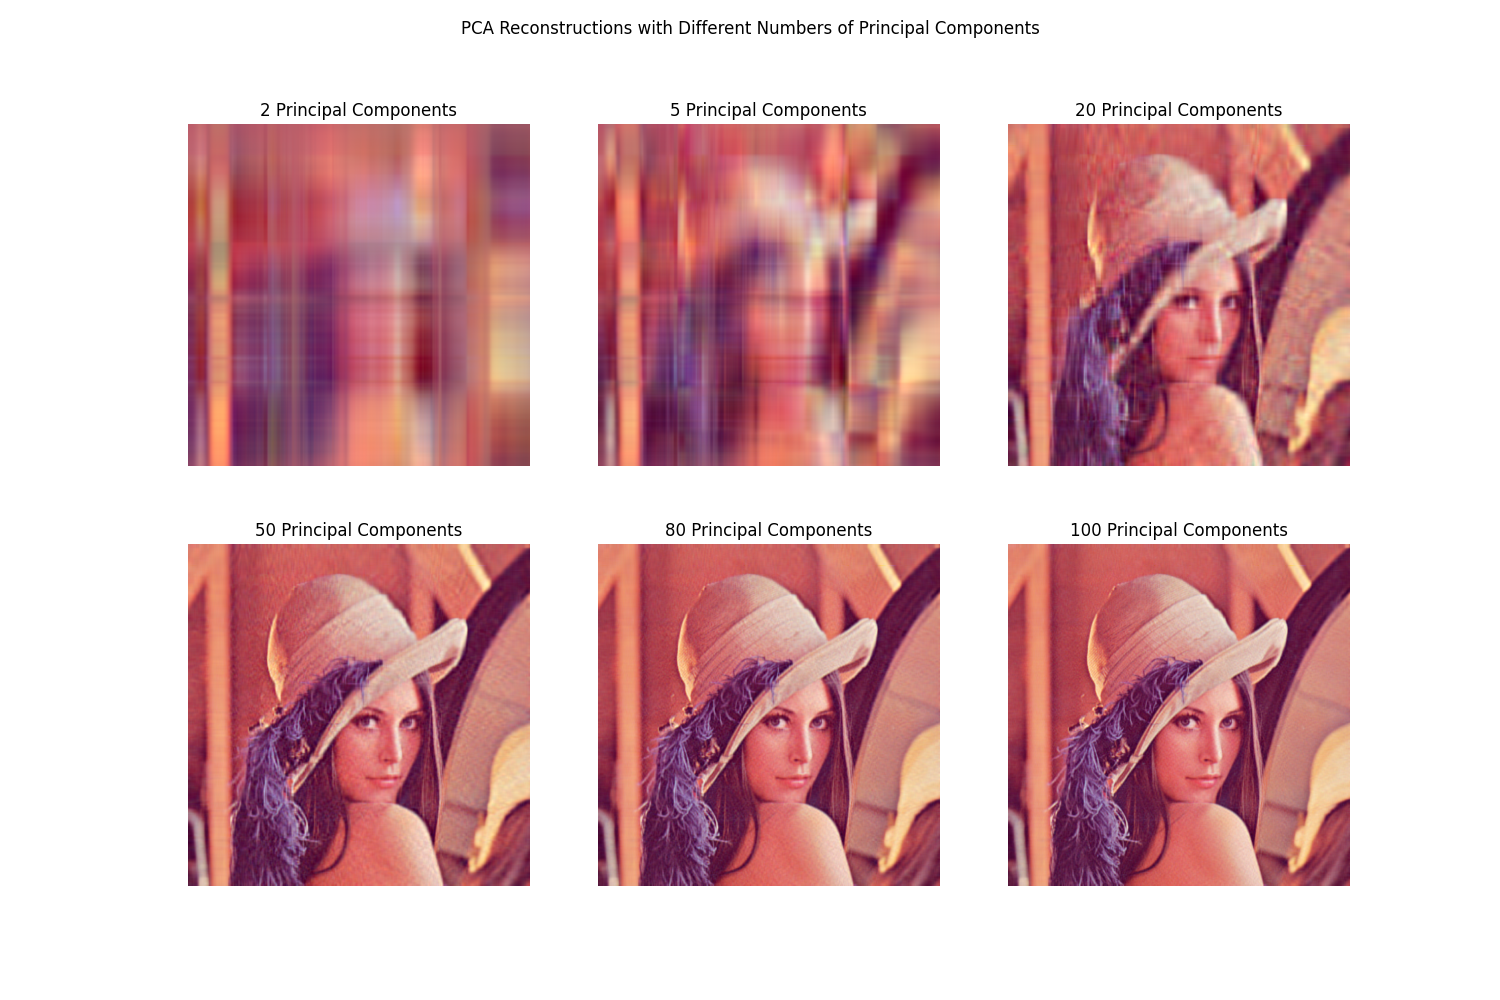
\includegraphics[width=\textwidth]{figures/hw3_1_1.png}
    	\caption{Reconstructed Lena Image Using 2, 5, 20, 50, 80, 100 Columns of U}
		\label{fig:reconstructed_lena}
\end{figure}

\begin{figure}[htbp]
    	\centering
    	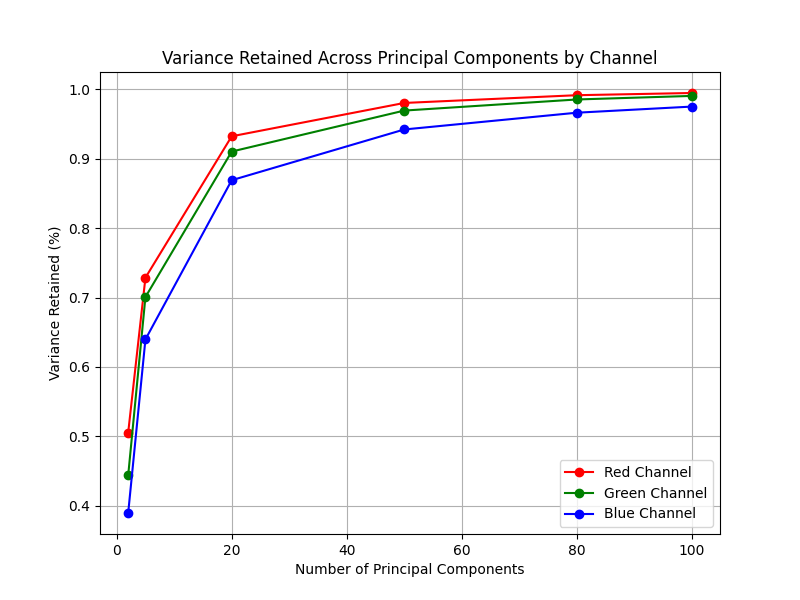
\includegraphics[width=\textwidth]{figures/hw3_1_2.png}
    	\caption{Variance of R,G,B Channels}
		\label{fig:variance_lena}
\end{figure}

\begin{verbatim}
	import numpy as np
	import matplotlib.pyplot as plt
	from skimage import io

	def recon(channel, nPC):
		# Perform SVD
		u, s, v = np.linalg.svd(channel, full_matrices=False)
		# Reconstruction using nPC columns
		picrecon = (u[:, :nPC] @ np.diag(s[:nPC]) @ v[:nPC, :])
		return picrecon

	def reconRGB(nPC):
		R_recon = recon(R, nPC)
		G_recon = recon(G, nPC)
		B_recon = recon(B, nPC)
		recon_img = np.stack((R_recon, G_recon, B_recon), axis=-1) + mean
		return np.clip(recon_img, 0, 1)

	def varPic(picArr):
		return np.var(picArr.reshape(-1, 3), axis=0)


	image_path = "Lenna.png"
	original = io.imread(image_path) / 255.0 
	pxl = original.reshape(-1, 3)
	mean = np.mean(pxl, axis=0)
	pxlCtr = pxl - mean
	R = pxlCtr[:, 0].reshape(512, 512)
	G = pxlCtr[:, 1].reshape(512, 512)
	B = pxlCtr[:, 2].reshape(512, 512)

	VarOrig = varPic(original)
	percentVar_R = []
	percentVar_G = []
	percentVar_B = []
	nPC_values = [2, 5, 20, 50, 80, 100]
	fig, axes = plt.subplots(2, 3, figsize=(15, 10))

	for ax, nPC in zip(axes.flat, nPC_values):
		recon_img = reconRGB(nPC)
		ax.imshow(recon_img)
		ax.set_title(f"{nPC} Principal Components")
		ax.axis('off')
		variance_retained = varPic(recon_img) / VarOrig
		percentVar_R.append(variance_retained[0])
		percentVar_G.append(variance_retained[1])
		percentVar_B.append(variance_retained[2])

	plt.suptitle("PCA Reconstructions with Different Numbers of Principal Components")
	plt.show()

	plt.figure(figsize=(8, 6))
	plt.plot(nPC_values, percentVar_R, color='red', marker='o', label='Red Channel')
	plt.plot(nPC_values, percentVar_G, color='green', marker='o', label='Green Channel')
	plt.plot(nPC_values, percentVar_B, color='blue', marker='o', label='Blue Channel')
	plt.xlabel("Number of Principal Components")
	plt.ylabel("Variance Retained (%)")
	plt.title("Variance Retained Across Principal Components by Channel")
	plt.legend()
	plt.grid(True)
	plt.show()
\end{verbatim}

	
		\newpage
	\section*{Problem 2}
	Let's revisit Least Squares Problem: $\minimize \limits_{\bm{\beta}} \frac{1}{2}\|\vy-\mA\bm{\beta}\|^2_2$, where $\mA\in\R^{n\times p}$.
	\begin{enumerate}
		\item Please show that if $p>n$, then vanilla solution $(\mA^T\mA)^{-1}\mA^T\vy$ is not applicable any more.	
		
		\textbf{Answer:}
		
		To demonstrate why the vanilla solution is not applicable when \( p > n \), take Singular Value Decomposition (SVD) of the matrix \(\mathbf{A} \in \mathbb{R}^{n \times p}\). 
		When \( p > n \), \(\mathbf{A}\) has more columns than rows, making it a wide matrix. We can decompose \(\mathbf{A}\) as follows:

		\[
		\mathbf{A} = \mathbf{U} \mathbf{\Sigma} \mathbf{V}^T,
		\]

		where:
		
		\(\mathbf{U} \in \mathbb{R}^{n \times n}\) is an orthogonal matrix,
		
		\(\mathbf{\Sigma} \in \mathbb{R}^{n \times p}\) is a rectangular diagonal matrix containing the singular values of \(\mathbf{A}\),
		
		\(\mathbf{V} \in \mathbb{R}^{p \times p}\) is an orthogonal matrix.

		Calculate \(\mathbf{A}^T \mathbf{A}\) using the SVD form of \(\mathbf{A}\):

		\[
		\mathbf{A}^T \mathbf{A} = (\mathbf{U} \mathbf{\Sigma} \mathbf{V}^T)^T (\mathbf{U} \mathbf{\Sigma} \mathbf{V}^T) = \mathbf{V} \mathbf{\Sigma}^T \mathbf{U}^T \mathbf{U} \mathbf{\Sigma} \mathbf{V}^T = \mathbf{V} \mathbf{\Sigma}^T \mathbf{\Sigma} \mathbf{V}^T.
		\]

		Since \(\mathbf{\Sigma} \in \mathbb{R}^{n \times p}\) is not square and has rank \(n\) (at most), \(\mathbf{\Sigma}^T \mathbf{\Sigma} \in \mathbb{R}^{p \times p}\) will also have rank \(n\), which is less than \(p\). This results in \(\mathbf{\Sigma}^T \mathbf{\Sigma}\) being singular, making \(\mathbf{A}^T \mathbf{A}\) singular as well.

		To illustrate this, note that for a matrix product \((\mathbf{A} \mathbf{B} \mathbf{C})^{-1} = \mathbf{C}^{-1} \mathbf{B}^{-1} \mathbf{A}^{-1}\), we would ideally find:

		\[
		(\mathbf{A}^T \mathbf{A})^{-1} = (\mathbf{V} \mathbf{\Sigma}^T \mathbf{\Sigma} \mathbf{V}^T)^{-1} = \mathbf{V} (\mathbf{\Sigma}^T \mathbf{\Sigma})^{-1} \mathbf{V}^T.
		\]

		However, since \(\mathbf{\Sigma}^T \mathbf{\Sigma}\) is not invertible (due to its rank deficiency), \((\mathbf{A}^T \mathbf{A})^{-1}\) does not exist. This non-invertibility leads to the inapplicability of the vanilla solution \((\mathbf{A}^T \mathbf{A})^{-1} \mathbf{A}^T \mathbf{y}\) when \(p > n\).
		
		\item Let's assume $\mA=[1, 2, 4;1, 3, 5; 1, 7, 7; 1, 8, 9], \vy=[1;2;3;4]$. Please show via experiment results that Gradient Descent method will obtain the optimal solution with  Linear Convergence rate if the learning rate is fixed to be $\frac{1}{\sigma_{max}(\mA^T\mA)}$, and $\bm{\beta}_0=[0;0;0]$.	
		
		\textbf{Answer:}
		In the next part (part 3), the learning rate for ridge regression is the same as the learning rate for this question (part 2) for $\lambda = 0$. Figure 3 shows the normalized objective scores as lambda is sweeped from 
		$\lambda = [0, 0.1, 1, 10, 100, 200]$
		As can be seen in Figure 3, the learning rates and convergence rates were highest when $\lambda = 0$.

		\item Now let's consider ridge regression: $\minimize \limits_{\bm{\beta}} \frac{1}{2}\|\vy-\mA\bm{\beta}\|^2_2+\frac{\lambda}{2} \|\bm{\beta}\|^2_2$, where  $\mA,\vy,\bm{\beta}_0$ remains the same as above while learning rate is fixed to be $\frac{1}{\lambda+\sigma_{max}(\mA^T\mA)}$ where $\lambda$ varies from $0.1,1,10,100,200$, please show that Gradient Descent method with larger $\lambda$ converges faster. 
		
		\textbf{Answer:}
		In Figure 3, a clear distinction is seen. As $\lambda$ increases, the learning and convergence rates decrease. This suggests that as $\lambda$ increases, there is faster convergence in shorter iterations. 

		\begin{figure}[htbp]
    		\centering
    		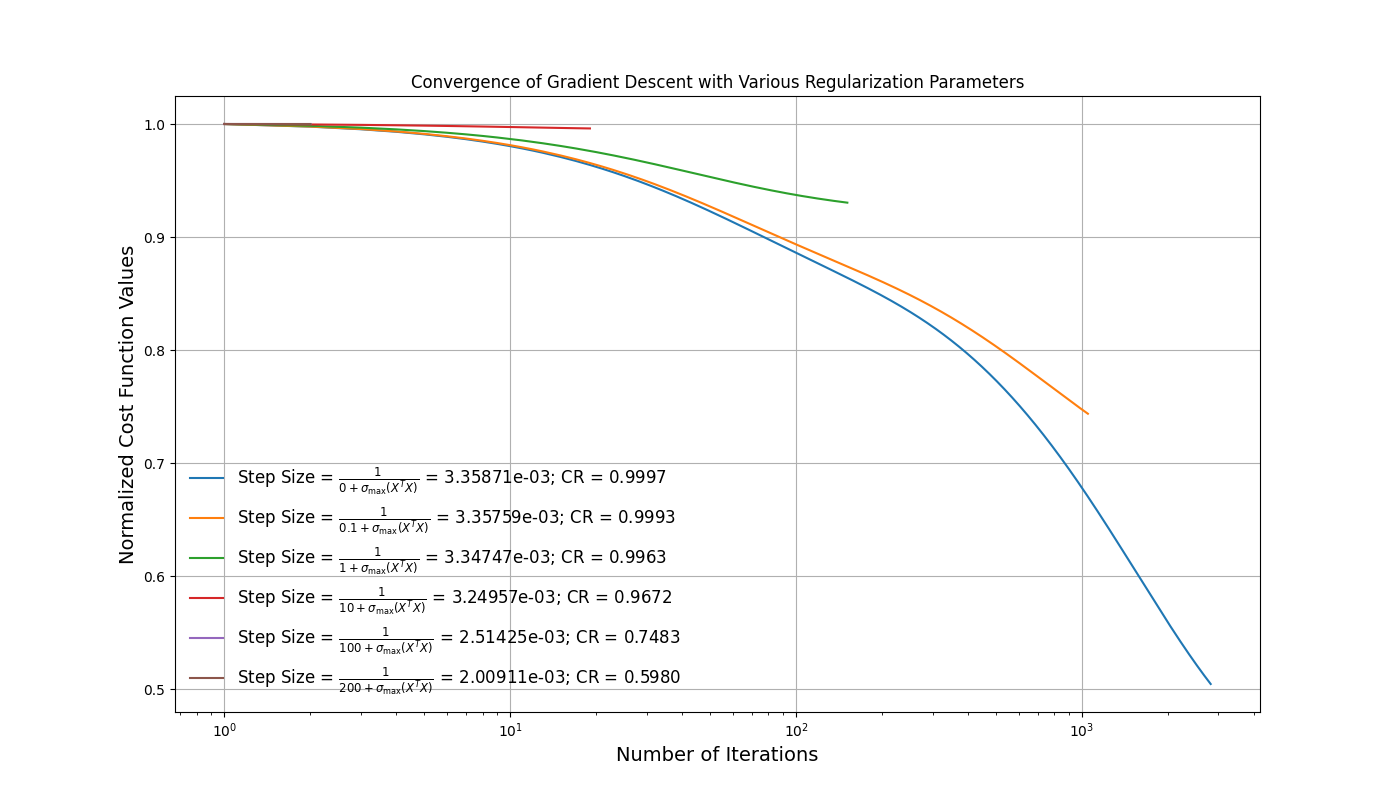
\includegraphics[width=\textwidth]{figures/hw3_2.png}
    		\caption{Object Scores vs Iterations as Lambda is Varied}
		\label{fig:objective_func_scores}
\end{figure}

	\end{enumerate}
	\begin{verbatim}
		import numpy as np
		import matplotlib.pyplot as plt
		import scipy.linalg as sl
		
		def cost_function(X, y, theta, reg_param):
			return ((X.dot(theta) - y).T.dot(X.dot(theta) - y) + reg_param * theta.T.dot(theta))[0][0] / 2
		
		def gradient(X, y, theta, reg_param):
			return X.T.dot(X.dot(theta) - y) + reg_param * theta
		
		def gradient_descent(cost_fn, grad_fn, X, y, init_theta, reg_param, step_size, tolerance):
			theta = init_theta
			iteration = 0
			delta = np.inf
			cost_history = [cost_fn(X, y, init_theta, reg_param)]
			while delta > tolerance:
				theta = theta - step_size * grad_fn(X, y, theta, reg_param)
				iteration += 1
				cost_history.append(cost_fn(X, y, theta, reg_param))
				delta = abs((cost_history[-1] - cost_history[-2]) / cost_history[-1])
			return iteration, theta, cost_history[1:]
		
		X = np.array([[1, 2, 4], [1, 3, 5], [1, 7, 7], [1, 8, 9]])
		y = np.array([[1], [2], [3], [4]])
		
		tolerance = 1e-4
		theta_init = np.zeros((3, 1))  
		regularization_params = [0, 0.1, 1, 10, 100, 200]  
		iterations_list = []  
		learning_rates = []  
		cost_values = []  
		convergence_ratios = []  
		
		for reg_param in regularization_params:
			step_size = 1 / (np.max(sl.svd(X.T.dot(X))[1]) + reg_param)
			iteration, _, cost_hist = gradient_descent(cost_function, gradient, X, y, theta_init, reg_param, step_size, tolerance)
			iterations_list.append(iteration)
			learning_rates.append(step_size)
			cost_values.append(cost_hist)
			_, singular_values, _ = sl.svd(X.T.dot(X) + reg_param * np.identity(3))
			convergence_ratios.append(1 - np.min(singular_values) / np.max(singular_values))
		
		cost_values = [cost_hist / cost_hist[0] for cost_hist in cost_values]
		
		plt.figure(figsize=(14, 8))
		for reg_param, iteration, cost_hist, lr, cr in zip(regularization_params, iterations_list, cost_values, learning_rates, convergence_ratios):
			plt.plot(np.arange(1, iteration + 1), cost_hist, 
					 label=fr'Step Size = $\frac{{1}}{{{reg_param} + \sigma_{{\max}}(X^T X)}}$ = {lr:.5e}; CR = {cr:.4f}')
		plt.xscale('log')
		plt.legend(frameon=False, fontsize=12)
		plt.xlabel('Number of Iterations', fontsize=14)
		plt.ylabel('Normalized Cost Function Values', fontsize=14)
		plt.title("Convergence of Gradient Descent with Various Regularization Parameters")
		plt.grid(True)
		plt.show()
	\end{verbatim}	
	\newpage
	
	\section*{Problem 3}
	We consider matrix completion problem. As we discussed in class, the main issue of \textit{softImpute (Matrix Completion via Iterative Soft-Thresholded SVD)} is when the matrix size is large, conducting \textit{SVD} is computational demanding. Let's recall the original problem where $\mX, \mZ \in\mathbb{R}^{n\times d}$: 
	\begin{equation}\label{eq:nuc}
	\min\limits_{\mZ}\frac{1}{2}\|P_\Omega(\mX)-P_\Omega(\mZ)\|_F^2+\lambda \|\mZ\|_*
	\end{equation} 
People have found that instead of finding optimal $\mZ$, it might be better to make use of \textit{Burer-Monteiro} method to optimize two matrices $\mA \in\mathbb{R}^{n\times r}, \mB\in\mathbb{R}^{d\times r} (r\ge rank(\mZ^*))$ such that $\mA\mB^T=\mZ$. The new objective is:
	\begin{equation}\label{eq:bur}
	\min\limits_{\mA,\mB}\frac{1}{2}\|P_\Omega(\mX-\mA\mB^T)\|_F^2+\frac{\lambda}{2}(\|\mA\|_F^2+\|\mB\|^2_F).
\end{equation} 
\begin{itemize}
	\item Assume $[\mU,\mSigma,\mV]=svd(\mZ)$, show that if $\mA=\mU\mSigma^\frac{1}{2}, \mB=\mV\mSigma^\frac{1}{2}$, then Eq. (\ref{eq:bur}) is equivalent to Eq. (\ref{eq:nuc}).
	
	\textbf{Answer:}

		Substitute \( \mathbf{A} \) and \( \mathbf{B} \) into \( \mathbf{Z} \):
		\[
		\mathbf{Z} = \mathbf{A} \mathbf{B}^T = (\mathbf{U} \mathbf{\Sigma}^{1/2})(\mathbf{V} \mathbf{\Sigma}^{1/2})^T = \mathbf{U} \mathbf{\Sigma}^{1/2} (\mathbf{\Sigma}^{1/2})^T \mathbf{V}^T = \mathbf{U} \mathbf{\Sigma} \mathbf{V}^T.
		\]
		This recovers the original matrix \( \mathbf{Z} = \mathbf{U} \mathbf{\Sigma} \mathbf{V}^T \), which is consistent with the requirement in Equation (1).

		Since \( \mathbf{A} = \mathbf{U} \mathbf{\Sigma}^{1/2} \), we have:
		\[
		\| \mathbf{A} \|_F^2 = \| \mathbf{U} \mathbf{\Sigma}^{1/2} \|_F^2 = \| \mathbf{\Sigma}^{1/2} \|_F^2 = \sum_{i} \sigma_i,
		\]
		where \( \sigma_i \) are the singular values of \( \mathbf{Z} \). Similarly, for \( \mathbf{B} = \mathbf{V} \mathbf{\Sigma}^{1/2} \), we obtain:
		\[
		\| \mathbf{B} \|_F^2 = \| \mathbf{\Sigma}^{1/2} \|_F^2 = \sum_{i} \sigma_i.
		\]
		Therefore,
		\[
		\frac{\lambda}{2} \left( \| \mathbf{A} \|_F^2 + \| \mathbf{B} \|_F^2 \right) = \lambda \sum_{i} \sigma_i = \lambda \| \mathbf{Z} \|_*,
		\]
		which matches the norm regularization term in the original objective (Equation 1).

		By substituting \( \mathbf{A} = \mathbf{U} \mathbf{\Sigma}^{1/2} \) and \( \mathbf{B} = \mathbf{V} \mathbf{\Sigma}^{1/2} \) in the new objective function:
		\[
		\min_{\mathbf{A}, \mathbf{B}} \frac{1}{2} \| \mathcal{P}_{\Omega}(\mathbf{X} - \mathbf{Z}) \|_F^2 + \lambda \| \mathbf{Z} \|_*,
		\]
		This is exactly the same as the original objective function in Equation (1).

		Thus, choosing \( \mathbf{A} = \mathbf{U} \mathbf{\Sigma}^{1/2} \) and \( \mathbf{B} = \mathbf{V} \mathbf{\Sigma}^{1/2} \) in Equation (2) makes the objective function equivalent to the original objective in Equation (1), as required.
		\item The \textit{Burer-Monteiro} method suggests if we can find  $\mA^*,\mB^*$, then the optimal $\mZ$ to Eq. (\ref{eq:nuc}) can be recovered by $\mA^*{\mB^*}^T$. It boils down to solve Eq. (\ref{eq:bur}). Show that we can make use of \text{least squares} with ridge regression to update $\mA, \mB$ row by row in an alternating minimization manner as below. Assume $n=d=2000, r=200$, please write program to find $\mZ^*$.
	\begin{algorithmic}
		\State $T \gets 100, i\gets 1$ \ \% \textcolor{blue}{you can also set T to be other number instead of 100}
		\If{$i\leq T$} 
			\State $update \ A \ row \ by \ row \ while \ fixing \ B$
			\State $update \ B \ row \ by \ row \ while \ fixing \ A$
			\State $i \gets i+1$
		%\EndIf
		\EndIf 
	\end{algorithmic}
	\end{itemize}

	\textbf{Answer: }

	Figure 4 shows the results of a python code that implements the \textit{Burer-Monteiro method} using an alternating minimization approach with ridge regression to find an approximate low-rank solution \( \mathbf{Z}^* = \mathbf{A} \mathbf{B}^T \) that closely matches a target matrix \( \mathbf{X} \). 
	The code alternates between updating each row of matrices \( \mathbf{A} \) and \( \mathbf{B} \) using ridge regression, iteratively reducing the approximation error until the solution converges.
	After the algorithm reaches the maximum number of iterations, the final approximation \( \mathbf{Z}^* = \mathbf{A} \mathbf{B}^T \) is computed. The code then calculates and prints the final relative approximation error between \( \mathbf{X} \) and \( \mathbf{Z}^* \), giving a measure of how well \( \mathbf{Z}^* \) approximates \( \mathbf{X} \).
	Figure 4 shows, the Forbenius Error between the approximated Z and ground truth X. After 100 iterations, the algorithm predicts a Z that aproximately equal to the ground truth. 


	\begin{verbatim}
		import numpy as np
		from sklearn.linear_model import Ridge
		import matplotlib.pyplot as plt
		
		n, d, r = 2000, 2000, 200  
		T = 100 
		lambda_ridge = 0.001  
		tolerance = 1e-6  
		np.random.seed(0)  
		
		A = np.random.randn(n, r) * 0.01 
		B = np.random.randn(d, r) * 0.01
		# Ground truth matrix X
		X = A @ B.T  
		
		def update_A(A, B, X, lambda_ridge):
			for i in range(n):
				ridge_reg = Ridge(alpha=lambda_ridge, fit_intercept=False)
				ridge_reg.fit(B, X[i, :])  
				A[i, :] = ridge_reg.coef_  
			return A
		
		def update_B(A, B, X, lambda_ridge):
			for j in range(d):
				ridge_reg = Ridge(alpha=lambda_ridge, fit_intercept=False)
				ridge_reg.fit(A, X[:, j])  
				B[j, :] = ridge_reg.coef_  
			return B
		
		frob_errors = []
		prev_error = None  
		
		for t in range(T):
			A = update_A(A, B, X, lambda_ridge)
			B = update_B(A, B, X, lambda_ridge)
			Z_current = A @ B.T
			frobenius_error = np.linalg.norm(X - Z_current, 'fro') / np.linalg.norm(X, 'fro')
			frob_errors.append(frobenius_error)
			print(f"Iteration {t + 1}, Frobenius error: {frobenius_error:.6f}")
			
		Z_star = A @ B.T
		print("Approximate solution Z* has been found.")
		
		plt.figure(figsize=(10, 6))
		plt.plot(range(1, len(frob_errors) + 1), frob_errors, marker='o', color='b')
		plt.xlabel('Iteration')
		plt.ylabel('Relative Frobenius Error')
		plt.title('Convergence of Frobenius Error Between X and Z*')
		plt.grid(True)
		plt.show()
		
	\end{verbatim}

\begin{figure}[htbp]
	\centering
	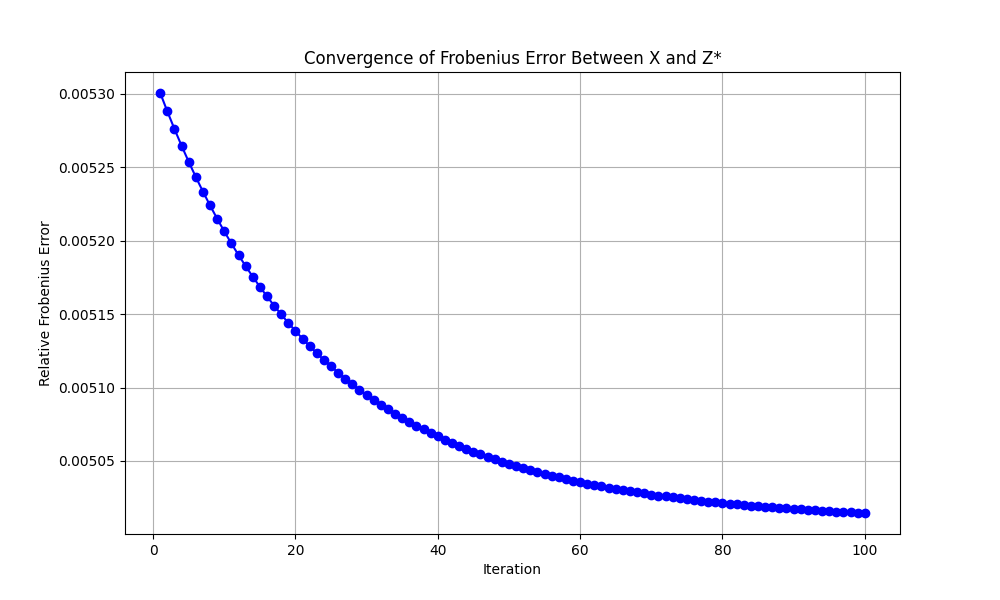
\includegraphics[width=\textwidth]{figures/hw3_3.png}
	\caption{Z* Approximation}
\label{fig:objective_func_scores}
\end{figure}

\end{document}
